\section{Metodología aplicada}
La metodología sigue la arquitectura y las puertas de validación descritas en la \textit{Guía Metodológica} (flujo funcional de la sección 1.1 y \textit{guardrails} de las secciones 4 y 6). PLAN\_01 organiza la definición y dependencias de las herramientas; PLAN\_02 describe su integración, selección de formulación, validación y comparación con referencias. Estos planes orientan el flujo, mientras que los resultados reportados proceden de los artefactos de la ejecución del circuito.

\begin{enumerate}
  \item \textbf{Entrada y alcance.} Se tomó el netlist \texttt{circuito\_objetivo.cir}, con referencia \texttt{0}, excitación AC de 1 mV y observable acordado $V(N OUT)/V(N IN)$ en el barrido lineal de 300 puntos entre 10 Hz y 100 kHz.
  \item \textbf{Puerta de validación del netlist.} \texttt{validate\_netlist.py} terminó en \textbf{Satisfactoriamente} con cero diagnósticos. Conforme a la metodología, un FAIL habría detenido el flujo antes de construir el circuito.
  \item \textbf{Parseo y modelo.} \texttt{parse\_netlist.py} generó la representación estructurada con valores en unidades SI. \texttt{build\_circuit\_model.py} conservó la identidad de componentes, el orden determinista de nodos y ramas y el op-amp como dispositivo aparte.
  \item \textbf{Topología.} \texttt{build\_oriented\_graph.py} produjo el grafo dirigido. \texttt{build\_incidence\_matrix.py} generó la matriz de incidencia reducida. La orientación sigue el orden de terminales del netlist y $+1/-1$ indica rama saliente/entrante, respectivamente.
  \item \textbf{Selección de formulación.} Debido a \texttt{.OPAMP U1 NP NM OUT IDEAL}, se eligió exclusivamente MNA. En el modelo lineal ideal del proyecto las corrientes de entrada son cero, $V(NP)=V(NM)$ y se incorpora una corriente auxiliar de salida. No se modelan rieles ni saturación; el op-amp no se sustituye por una rama pasiva.
  \item \textbf{Ensamble y barrido.} \texttt{build\_mna\_system.py} produjo el sistema complejo MNA de $7\times7$ para 10 Hz. \texttt{solve\_ac\_sweep.py} ejecutó el barrido completo en MNA y produjo las transferencias, magnitudes, dB y fases por frecuencia.
  \item \textbf{Validación de solución.} Se revisaron estados de solver y validación en cada frecuencia. El resultado fue \textbf{Satisfactorio} globalmente en los 300 puntos; el residuo lineal reportado varió entre $1.59\times10^{-24}$ y $5.16\times10^{-20}$. La solución sólo se considera aceptada por este estado y por los controles internos reportados.
  \item \textbf{Comparación externa y presentación.} Se usó el listado HSPICE existente como referencia, sin interpolar frecuencias. \texttt{compare\_reference.py} comparó únicamente los dos puntos con frecuencia exactamente coincidente (10 Hz y 100 kHz); ambos pasaron con las tolerancias declaradas en el artefacto. Luego se incorporaron la topología y las gráficas de los resultados disponibles.
\end{enumerate}

\begin{figure}[H]
\centering
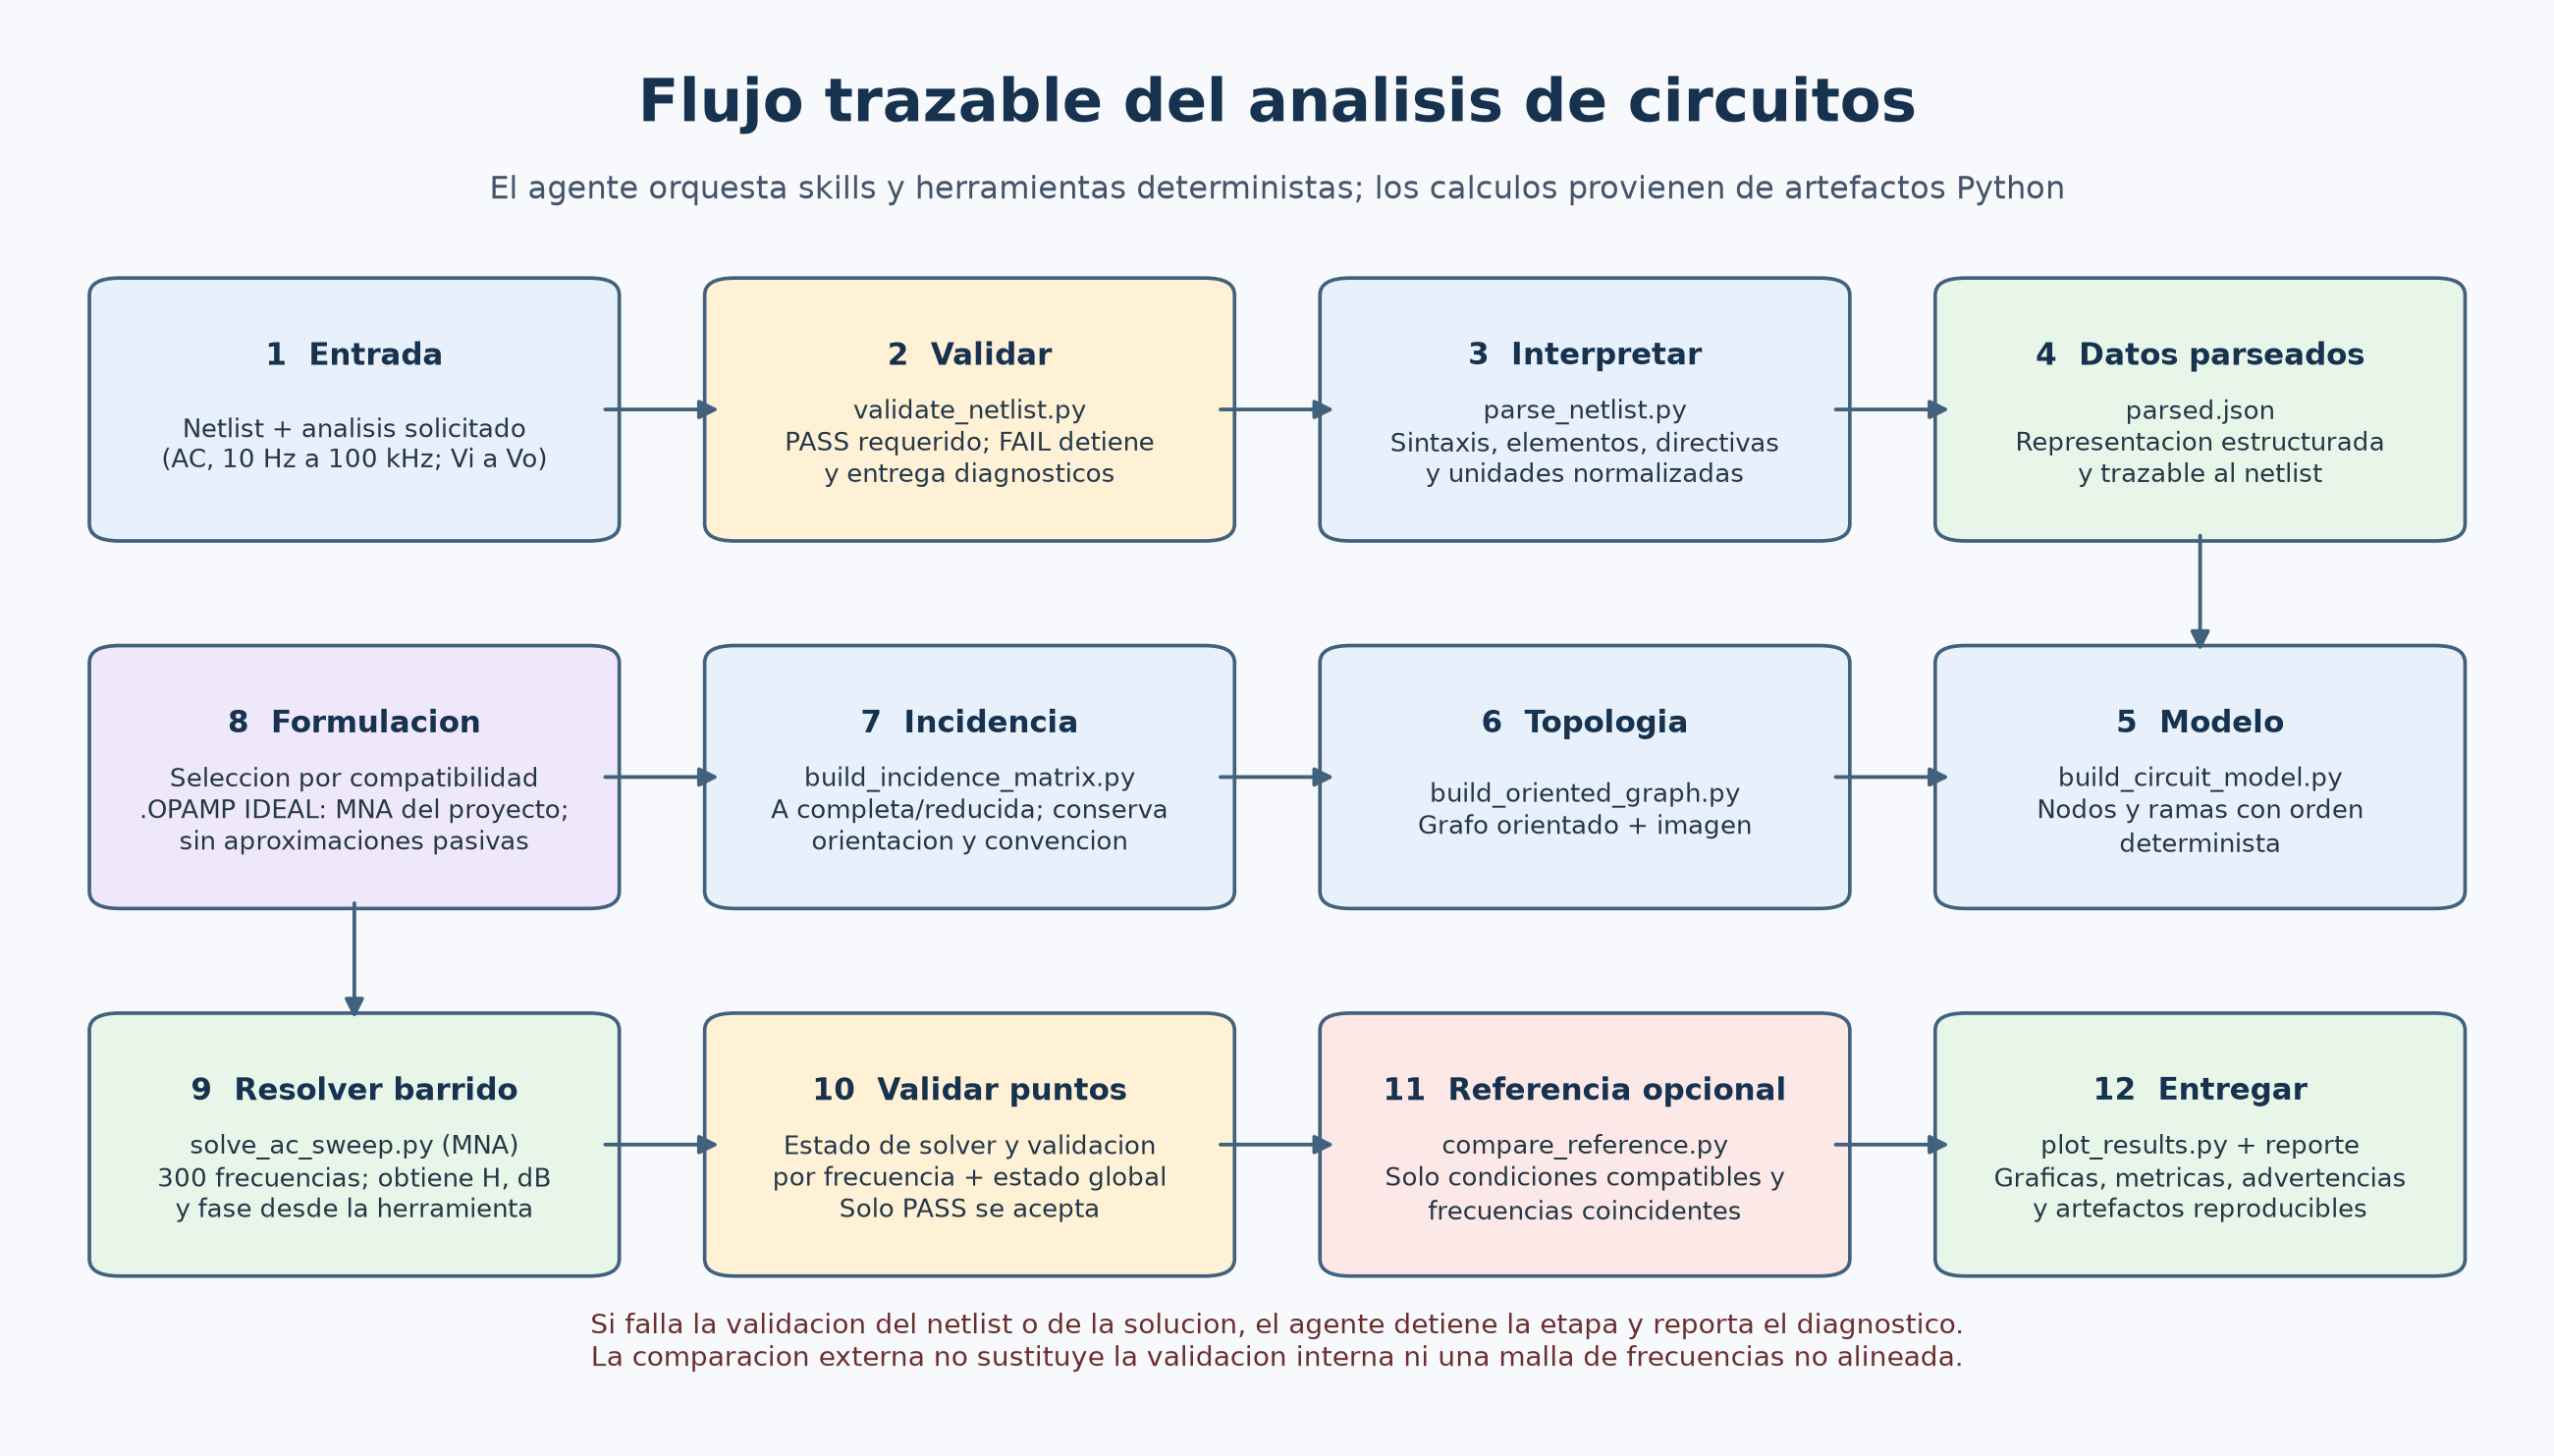
\includegraphics[scale=0.35]{flujo_analisis_agente.png}
\caption{Etapas del agente: validación, construcción del modelo, formulación, resolución, verificación y entrega. Las puertas en FAIL detienen el flujo.}
\end{figure}